\subsection{Performance}

El algoritmo que dise\'niamos se comporta exactamente igual para cualquier tipo de instancia v\'alida que tenga como entrada. Al no aplicar ninguna m\'inima heur\'isticano reducimos ning\'un calculo ni aprobechamos alguna informaci\'on particular de la entrada.

Con lo cual el desempe\'no del algoritmo depende pura y exclusivamente de las dos variables que se manejan en la instancio. El tama\'no del tablero que repercute en el modelado del grafo y la cantidad de nodos totales y nodos en la lista de adyacencia de los nodos, y la cantidad de caballos que impl\'ica la cantidad de BFS que se corren.

Un optimizaci\'on sencilla que se podr\'ia realizar y no se hizo por falta de tiempo es que en vez de tener una lista de caballos, utilizar un mapa<Caballo,Cantidad>, que representa la cantidad de caballos que hay en una misma casilla al comienzo.
Con lo cual en el BFS en vez de contemplar el movimiento de un solo caballo lo hago con la cantidad de caballos que comiencen en esa casilla. Lo cual me reduce cantidad de caballos BFS a la hora de computarlos.

Para todos los experimentos la posici\'on inicial de los caballos se seleccion\'o aleatoreamente con posiciones v\'alidas dentro de los tableros utilizados.


En la primer imagen fijamos a la cantidad de caballos en 50 y modificamos el tama\'no de la matriz. Y como podemos apreciar obtuvimos una funcion cuadr\'atica como era de esperarse.

\begin{figure}[H]
\begin{center}
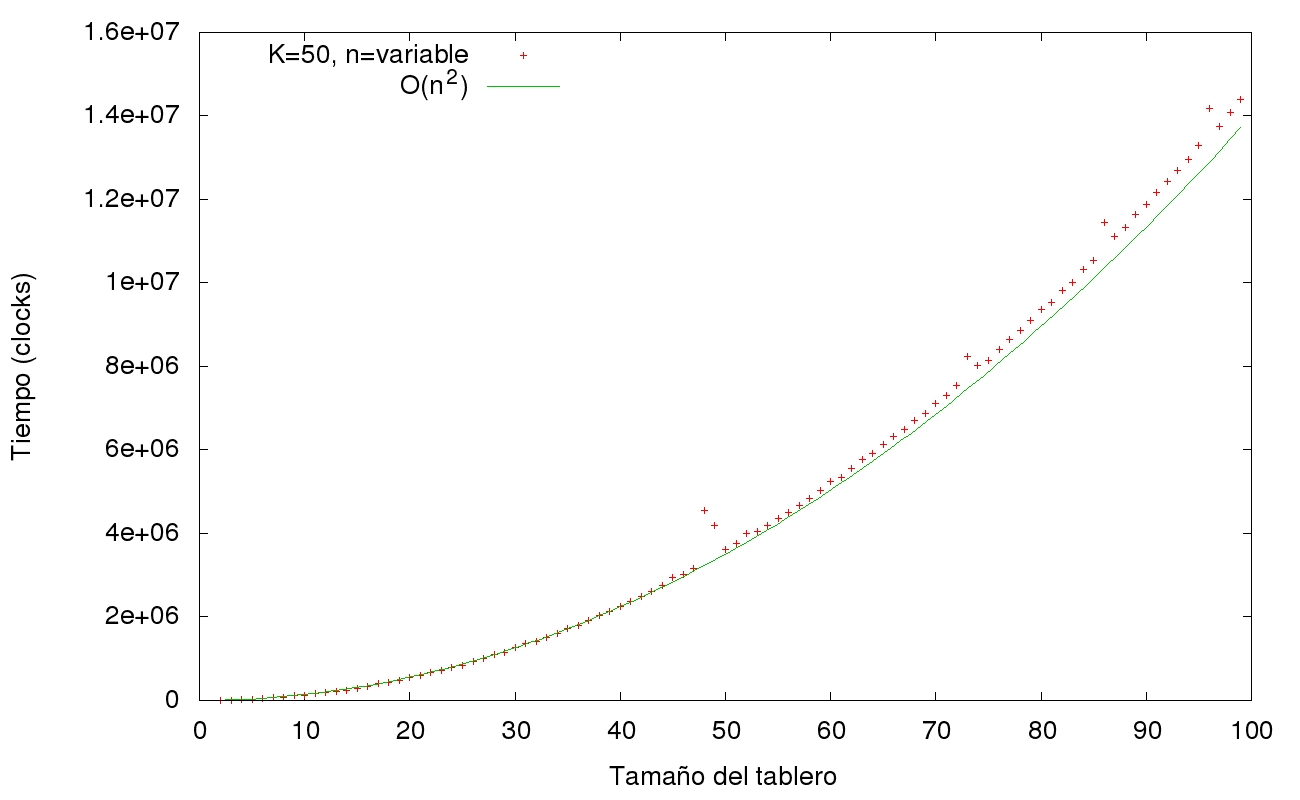
\includegraphics[scale=0.35]{./imagenes/ej2_chartRendimiento.png}
\caption{K f\'ijo en 50 y N variando de 1 a 100}
\end{center}
\end{figure}

Luego dejamos f\'ijo N en 70 e hicimos variar la cantidad de caballos desde 1 a 100 y como se observa a continuaci\'on obtuvimos una l\'ineal.

\begin{figure}[H]
\begin{center}
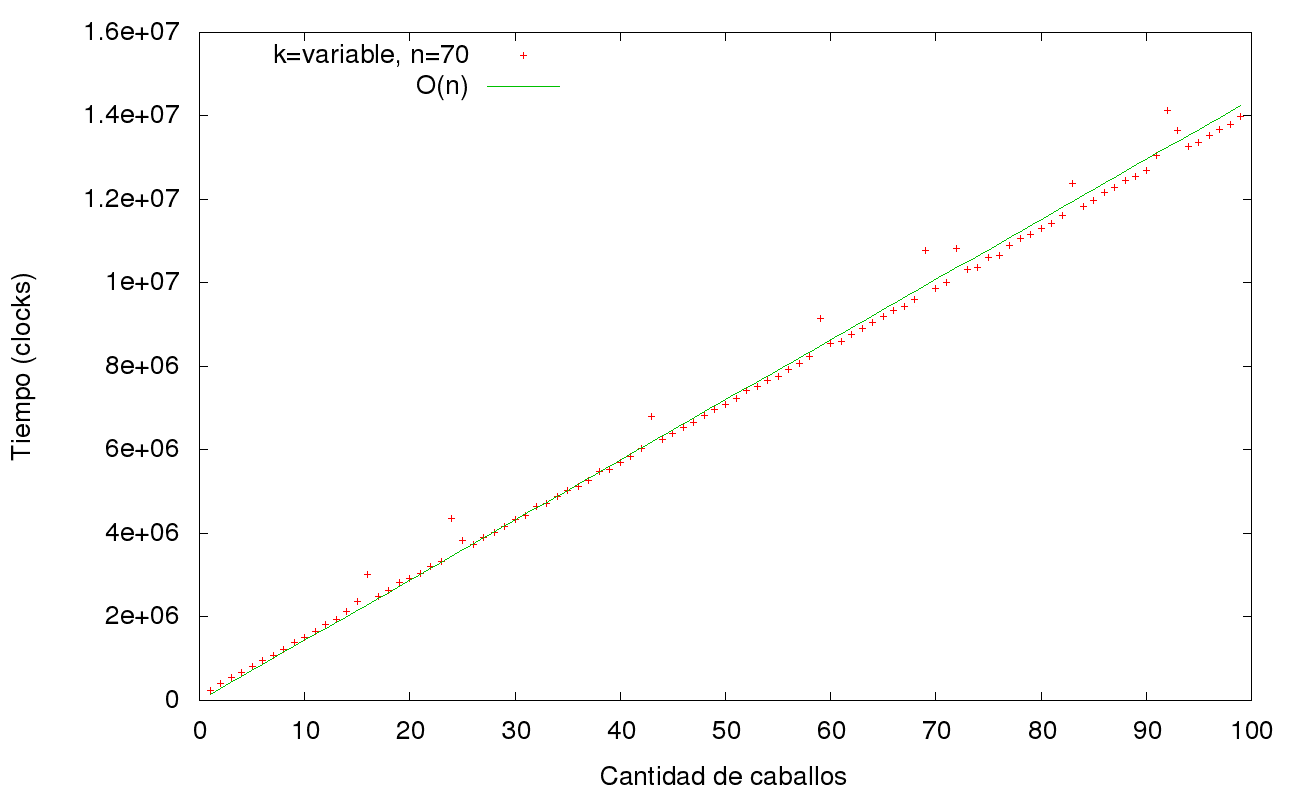
\includegraphics[scale=0.35]{./imagenes/ej2_chartRendimiento2.png}
\caption{N f\'ijo en 70 y K variando de 1 a 100.}
\end{center}
\end{figure}

Por \'ultimo realizamos un test en donde incrementamos gradualmente la cantidad de caballos y el tama\'no de la matriz simultaneamente. Con lo cual la funci\'on que obtuvimos es c\'ubica pues $k = n$ y los dos fueron desde 1 a 100.


\begin{figure}[H]
\begin{center}
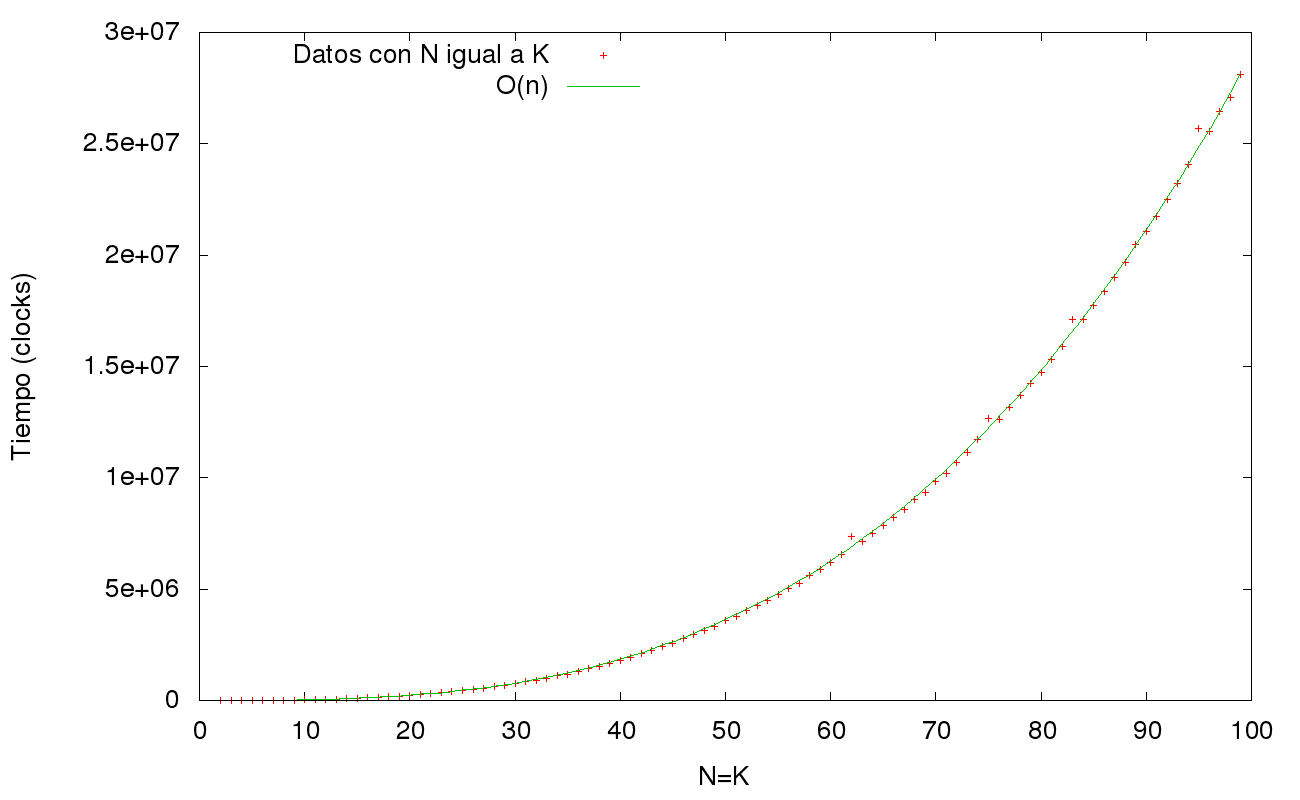
\includegraphics[scale=0.35]{./imagenes/ej2_chartRendimiento3.png}
\caption{K y N variando de 1 a 100 los dos simultaneamente.}
\end{center}
\end{figure}